\documentclass{article}

\usepackage[margin=0.5in]{geometry}
\usepackage{enumitem}
\usepackage{graphicx}

\title{2.1 Statistics and Probability Homework}
\author{}
\date{}

\begin{document}
\maketitle

\begin{enumerate}[resume]
    % AMC 8, 2020 Problem 13
    \item Jamal has a drawer containing $6$ green socks, $18$ purple socks, and $12$ orange socks.
        After adding more purple socks, Jamal noticed that there is now a $60\%$ chance that a sock randomly selected from the drawer is purple.
        How many purple socks did Jamal add?
        \vspace{3cm}
    % AMC 8, 2019 Problem 18
    \item The faces of each of two fair dice are numbered $1$, $2$, $3$, $5$, $7$, and $8$.
        When the two dice are tossed, what is the probability that their sum will be an even number?
        \vspace{3cm}
    % AMC 8, 2006 Problem 17
    \item Jeff rotates spinners $P$, $Q$ and $R$ and adds the resulting numbers.
        What is the probability that his sum is an odd number?
        \begin{center}
            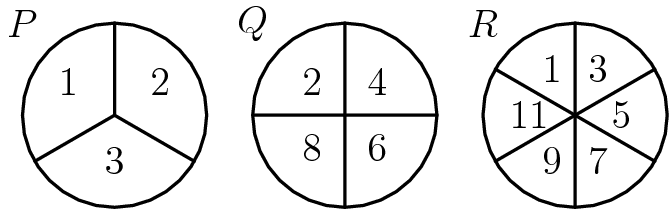
\includegraphics[scale=0.25]{spinners.png}
        \end{center}
        \vspace{2cm}
    % AMC 8, 2019 Problem 7
    \item Shauna takes five tests, each worth a maximum of $100$ points.
        Her scores on the first three tests are $76$, $94$, and $87$.
        In order to average $81$ for all five tests, what is the lowest score she could earn on one of the other two tests?
        \vspace{3cm}
    % AMC 8, 2018 Problem 23
    \item From a regular octagon, a triangle is formed by connecting three randomly chosen vertices of the octagon.
        What is the probability that at least one of the sides of the triangle is also a side of the octagon?
        \begin{center}
            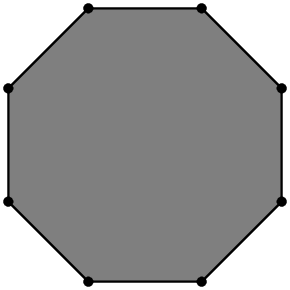
\includegraphics[scale=0.25]{octagon.png}
        \end{center}
\end{enumerate}
\end{document}